%% bare_conf_compsoc.tex
%% V1.4b
%% 2015/08/26
%% by Michael Shell
%% See:
%% http://www.michaelshell.org/
%% for current contact information.
%%
%% This is a skeleton file demonstrating the use of IEEEtran.cls
%% (requires IEEEtran.cls version 1.8b or later) with an IEEE Computer
%% Society conference paper.
%%
%% Support sites:
%% http://www.michaelshell.org/tex/ieeetran/
%% http://www.ctan.org/pkg/ieeetran
%% and
%% http://www.ieee.org/

%%*************************************************************************
%% Legal Notice:
%% This code is offered as-is without any warranty either expressed or
%% implied; without even the implied warranty of MERCHANTABILITY or
%% FITNESS FOR A PARTICULAR PURPOSE! 
%% User assumes all risk.
%% In no event shall the IEEE or any contributor to this code be liable for
%% any damages or losses, including, but not limited to, incidental,
%% consequential, or any other damages, resulting from the use or misuse
%% of any information contained here.
%%
%% All comments are the opinions of their respective authors and are not
%% necessarily endorsed by the IEEE.
%%
%% This work is distributed under the LaTeX Project Public License (LPPL)
%% ( http://www.latex-project.org/ ) version 1.3, and may be freely used,
%% distributed and modified. A copy of the LPPL, version 1.3, is included
%% in the base LaTeX documentation of all distributions of LaTeX released
%% 2003/12/01 or later.
%% Retain all contribution notices and credits.
%% ** Modified files should be clearly indicated as such, including  **
%% ** renaming them and changing author support contact information. **
%%*************************************************************************


% *** Authors should verify (and, if needed, correct) their LaTeX system  ***
% *** with the testflow diagnostic prior to trusting their LaTeX platform ***
% *** with production work. The IEEE's font choices and paper sizes can   ***
% *** trigger bugs that do not appear when using other class files.       ***                          ***
% The testflow support page is at:
% http://www.michaelshell.org/tex/testflow/



\documentclass[conference,compsoc]{IEEEtran}
% Some/most Computer Society conferences require the compsoc mode option,
% but others may want the standard conference format.
%
% If IEEEtran.cls has not been installed into the LaTeX system files,
% manually specify the path to it like:
% \documentclass[conference,compsoc]{../sty/IEEEtran}





% Some very useful LaTeX packages include:
% (uncomment the ones you want to load)


% *** MISC UTILITY PACKAGES ***
%

\usepackage[utf8x]{inputenc}
\usepackage[T1]{fontenc}
\usepackage{tikz, pgfplots}

%\usepackage{ifpdf}
% Heiko Oberdiek's ifpdf.sty is very useful if you need conditional
% compilation based on whether the output is pdf or dvi.
% usage:
% \ifpdf
%   % pdf code
% \else
%   % dvi code
% \fi
% The latest version of ifpdf.sty can be obtained from:
% http://www.ctan.org/pkg/ifpdf
% Also, note that IEEEtran.cls V1.7 and later provides a builtin
% \ifCLASSINFOpdf conditional that works the same way.
% When switching from latex to pdflatex and vice-versa, the compiler may
% have to be run twice to clear warning/error messages.






% *** CITATION PACKAGES ***
%
\ifCLASSOPTIONcompsoc
  % IEEE Computer Society needs nocompress option
  % requires cite.sty v4.0 or later (November 2003)
  \usepackage[nocompress]{cite}
\else
  % normal IEEE
  \usepackage{cite}
\fi
% cite.sty was written by Donald Arseneau
% V1.6 and later of IEEEtran pre-defines the format of the cite.sty package
% \cite{} output to follow that of the IEEE. Loading the cite package will
% result in citation numbers being automatically sorted and properly
% "compressed/ranged". e.g., [1], [9], [2], [7], [5], [6] without using
% cite.sty will become [1], [2], [5]--[7], [9] using cite.sty. cite.sty's
% \cite will automatically add leading space, if needed. Use cite.sty's
% noadjust option (cite.sty V3.8 and later) if you want to turn this off
% such as if a citation ever needs to be enclosed in parenthesis.
% cite.sty is already installed on most LaTeX systems. Be sure and use
% version 5.0 (2009-03-20) and later if using hyperref.sty.
% The latest version can be obtained at:
% http://www.ctan.org/pkg/cite
% The documentation is contained in the cite.sty file itself.
%
% Note that some packages require special options to format as the Computer
% Society requires. In particular, Computer Society  papers do not use
% compressed citation ranges as is done in typical IEEE papers
% (e.g., [1]-[4]). Instead, they list every citation separately in order
% (e.g., [1], [2], [3], [4]). To get the latter we need to load the cite
% package with the nocompress option which is supported by cite.sty v4.0
% and later.





% *** GRAPHICS RELATED PACKAGES ***
%
\ifCLASSINFOpdf
  % \usepackage[pdftex]{graphicx}
  % declare the path(s) where your graphic files are
  % \graphicspath{{../pdf/}{../jpeg/}}
  % and their extensions so you won't have to specify these with
  % every instance of \includegraphics
  % \DeclareGraphicsExtensions{.pdf,.jpeg,.png}
\else
  % or other class option (dvipsone, dvipdf, if not using dvips). graphicx
  % will default to the driver specified in the system graphics.cfg if no
  % driver is specified.
  % \usepackage[dvips]{graphicx}
  % declare the path(s) where your graphic files are
  % \graphicspath{{../eps/}}
  % and their extensions so you won't have to specify these with
  % every instance of \includegraphics
  % \DeclareGraphicsExtensions{.eps}
\fi
% graphicx was written by David Carlisle and Sebastian Rahtz. It is
% required if you want graphics, photos, etc. graphicx.sty is already
% installed on most LaTeX systems. The latest version and documentation
% can be obtained at: 
% http://www.ctan.org/pkg/graphicx
% Another good source of documentation is "Using Imported Graphics in
% LaTeX2e" by Keith Reckdahl which can be found at:
% http://www.ctan.org/pkg/epslatex
%
% latex, and pdflatex in dvi mode, support graphics in encapsulated
% postscript (.eps) format. pdflatex in pdf mode supports graphics
% in .pdf, .jpeg, .png and .mps (metapost) formats. Users should ensure
% that all non-photo figures use a vector format (.eps, .pdf, .mps) and
% not a bitmapped formats (.jpeg, .png). The IEEE frowns on bitmapped formats
% which can result in "jaggedy"/blurry rendering of lines and letters as
% well as large increases in file sizes.
%
% You can find documentation about the pdfTeX application at:
% http://www.tug.org/applications/pdftex





% *** MATH PACKAGES ***
%
\usepackage{amsmath}
% A popular package from the American Mathematical Society that provides
% many useful and powerful commands for dealing with mathematics.
%
% Note that the amsmath package sets \interdisplaylinepenalty to 10000
% thus preventing page breaks from occurring within multiline equations. Use:
%\interdisplaylinepenalty=2500
% after loading amsmath to restore such page breaks as IEEEtran.cls normally
% does. amsmath.sty is already installed on most LaTeX systems. The latest
% version and documentation can be obtained at:
% http://www.ctan.org/pkg/amsmath





% *** SPECIALIZED LIST PACKAGES ***
%
%\usepackage{algorithmic}
% algorithmic.sty was written by Peter Williams and Rogerio Brito.
% This package provides an algorithmic environment fo describing algorithms.
% You can use the algorithmic environment in-text or within a figure
% environment to provide for a floating algorithm. Do NOT use the algorithm
% floating environment provided by algorithm.sty (by the same authors) or
% algorithm2e.sty (by Christophe Fiorio) as the IEEE does not use dedicated
% algorithm float types and packages that provide these will not provide
% correct IEEE style captions. The latest version and documentation of
% algorithmic.sty can be obtained at:
% http://www.ctan.org/pkg/algorithms
% Also of interest may be the (relatively newer and more customizable)
% algorithmicx.sty package by Szasz Janos:
% http://www.ctan.org/pkg/algorithmicx




% *** ALIGNMENT PACKAGES ***
%
%\usepackage{array}
% Frank Mittelbach's and David Carlisle's array.sty patches and improves
% the standard LaTeX2e array and tabular environments to provide better
% appearance and additional user controls. As the default LaTeX2e table
% generation code is lacking to the point of almost being broken with
% respect to the quality of the end results, all users are strongly
% advised to use an enhanced (at the very least that provided by array.sty)
% set of table tools. array.sty is already installed on most systems. The
% latest version and documentation can be obtained at:
% http://www.ctan.org/pkg/array


% IEEEtran contains the IEEEeqnarray family of commands that can be used to
% generate multiline equations as well as matrices, tables, etc., of high
% quality.




% *** SUBFIGURE PACKAGES ***
%\ifCLASSOPTIONcompsoc
%  \usepackage[caption=false,font=footnotesize,labelfont=sf,textfont=sf]{subfig}
%\else
%  \usepackage[caption=false,font=footnotesize]{subfig}
%\fi
% subfig.sty, written by Steven Douglas Cochran, is the modern replacement
% for subfigure.sty, the latter of which is no longer maintained and is
% incompatible with some LaTeX packages including fixltx2e. However,
% subfig.sty requires and automatically loads Axel Sommerfeldt's caption.sty
% which will override IEEEtran.cls' handling of captions and this will result
% in non-IEEE style figure/table captions. To prevent this problem, be sure
% and invoke subfig.sty's "caption=false" package option (available since
% subfig.sty version 1.3, 2005/06/28) as this is will preserve IEEEtran.cls
% handling of captions.
% Note that the Computer Society format requires a sans serif font rather
% than the serif font used in traditional IEEE formatting and thus the need
% to invoke different subfig.sty package options depending on whether
% compsoc mode has been enabled.
%
% The latest version and documentation of subfig.sty can be obtained at:
% http://www.ctan.org/pkg/subfig




% *** FLOAT PACKAGES ***
%
%\usepackage{fixltx2e}
% fixltx2e, the successor to the earlier fix2col.sty, was written by
% Frank Mittelbach and David Carlisle. This package corrects a few problems
% in the LaTeX2e kernel, the most notable of which is that in current
% LaTeX2e releases, the ordering of single and double column floats is not
% guaranteed to be preserved. Thus, an unpatched LaTeX2e can allow a
% single column figure to be placed prior to an earlier double column
% figure.
% Be aware that LaTeX2e kernels dated 2015 and later have fixltx2e.sty's
% corrections already built into the system in which case a warning will
% be issued if an attempt is made to load fixltx2e.sty as it is no longer
% needed.
% The latest version and documentation can be found at:
% http://www.ctan.org/pkg/fixltx2e


%\usepackage{stfloats}
% stfloats.sty was written by Sigitas Tolusis. This package gives LaTeX2e
% the ability to do double column floats at the bottom of the page as well
% as the top. (e.g., "\begin{figure*}[!b]" is not normally possible in
% LaTeX2e). It also provides a command:
%\fnbelowfloat
% to enable the placement of footnotes below bottom floats (the standard
% LaTeX2e kernel puts them above bottom floats). This is an invasive package
% which rewrites many portions of the LaTeX2e float routines. It may not work
% with other packages that modify the LaTeX2e float routines. The latest
% version and documentation can be obtained at:
% http://www.ctan.org/pkg/stfloats
% Do not use the stfloats baselinefloat ability as the IEEE does not allow
% \baselineskip to stretch. Authors submitting work to the IEEE should note
% that the IEEE rarely uses double column equations and that authors should try
% to avoid such use. Do not be tempted to use the cuted.sty or midfloat.sty
% packages (also by Sigitas Tolusis) as the IEEE does not format its papers in
% such ways.
% Do not attempt to use stfloats with fixltx2e as they are incompatible.
% Instead, use Morten Hogholm'a dblfloatfix which combines the features
% of both fixltx2e and stfloats:
%
% \usepackage{dblfloatfix}
% The latest version can be found at:
% http://www.ctan.org/pkg/dblfloatfix




% *** PDF, URL AND HYPERLINK PACKAGES ***
%
%\usepackage{url}
\usepackage{hyperref}
% url.sty was written by Donald Arseneau. It provides better support for
% handling and breaking URLs. url.sty is already installed on most LaTeX
% systems. The latest version and documentation can be obtained at:
% http://www.ctan.org/pkg/url
% Basically, \url{my_url_here}.




% *** Do not adjust lengths that control margins, column widths, etc. ***
% *** Do not use packages that alter fonts (such as pslatex).         ***
% There should be no need to do such things with IEEEtran.cls V1.6 and later.
% (Unless specifically asked to do so by the journal or conference you plan
% to submit to, of course. )


% correct bad hyphenation here
\hyphenation{op-tical net-works semi-conduc-tor}


\begin{document}
%
% paper title
% Titles are generally capitalized except for words such as a, an, and, as,
% at, but, by, for, in, nor, of, on, or, the, to and up, which are usually
% not capitalized unless they are the first or last word of the title.
% Linebreaks \\ can be used within to get better formatting as desired.
% Do not put math or special symbols in the title.
\title{Two approaches to reduce the rank reversal occurrences in the  \textsc{promethee ii} method} 


% author names and affiliations
% use a multiple column layout for up to three different
% affiliations
\author{\IEEEauthorblockN{Dejaegere Gilles}
\IEEEauthorblockA{Synthèse du mémoire présenté en vue de l’obtention du diplôme\\ 
    d'Ingénieur Civil Informaticien à finalité spécialisée \\
}}
% conference papers do not typically use \thanks and this command
% is locked out in conference mode. If really needed, such as for
% the acknowledgment of grants, issue a \IEEEoverridecommandlockouts
% after \documentclass

% for over three affiliations, or if they all won't fit within the width
% of the page (and note that there is less available width in this regard for
% compsoc conferences compared to traditional conferences), use this
% alternative format:
% 
%\author{\IEEEauthorblockN{Michael Shell\IEEEauthorrefmark{1},
%Homer Simpson\IEEEauthorrefmark{2},
%James Kirk\IEEEauthorrefmark{3}, 
%Montgomery Scott\IEEEauthorrefmark{3} and
%Eldon Tyrell\IEEEauthorrefmark{4}}
%\IEEEauthorblockA{\IEEEauthorrefmark{1}School of Electrical and Computer Engineering\\
%Georgia Institute of Technology,
%Atlanta, Georgia 30332--0250\\ Email: see http://www.michaelshell.org/contact.html}
%\IEEEauthorblockA{\IEEEauthorrefmark{2}Twentieth Century Fox, Springfield, USA\\
%Email: homer@thesimpsons.com}
%\IEEEauthorblockA{\IEEEauthorrefmark{3}Starfleet Academy, San Francisco, California 96678-2391\\
%Telephone: (800) 555--1212, Fax: (888) 555--1212}
%\IEEEauthorblockA{\IEEEauthorrefmark{4}Tyrell Inc., 123 Replicant Street, Los Angeles, California 90210--4321}}




% use for special paper notices
%\IEEEspecialpapernotice{(Invited Paper)}




% make the title area
\maketitle

% As a general rule, do not put math, special symbols or citations
% in the abstract
%\begin{abstract}
%The abstract goes here.
%\end{abstract}

% no keywords




% For peer review papers, you can put extra information on the cover
% page as needed:
% \ifCLASSOPTIONpeerreview
% \begin{center} \bfseries EDICS Category: 3-BBND \end{center}
% \fi
%
% For peerreview papers, this IEEEtran command inserts a page break and
% creates the second title. It will be ignored for other modes.
\IEEEpeerreviewmaketitle



\section{Introduction}

%In a world as wide and complex as ours, finding optimal solutions to our decision problems has become a fastidious task.
In a world as wide and complex as ours, one is often confronted to intricate and complex decision problems. 
These problems often consist of different conflicting aspects which should simultaneously be optimised.
Unfortunately, there is generally no optimal solution which optimises all these aspects and choosing a best solution therefore consist in making the best trade-off. 
Finding these trade-offs can be a fastidious task and making a non optimal choice could lead to dramatic consequences.
Therefore, the entity in charge of the decision (called the decision maker) could want to use some multi-criteria decision aid methods. These methods are aimed at giving the decision maker some insights about the problem by elaborating a mathematical model and quantifying the different solutions.

% In the rest of this article, a decision problem will formalised as \cite{Bertrand2002}:
% 
% \begin{equation}
%     Opt \  \{f_1(a_i), \cdots , f_c(a_i), \cdots , f_k(a_i) | a_i \in A\}
%     \label{eq:multicriteria_pb_model}
% \end{equation}
% 
% \noindent With:
% \begin{description}
%     \item[$A$: ]  the set of all the possible solutions (or alternatives) of the decision problem. The size of this set will be denoted by $n$.
%     \item[$f_c$:] one of the $k$ evaluation function representing a the criteria on which the alternatives are evaluated.
% \end{description}
 
\section{\textsc{promethee ii} and rank reversals}
One of these multi-criteria decision aid methods is \textsc{promethee ii} (Preference Ranking Organisation METHod for Enrichment Evaluations) which has originally been proposed by J.P. Brans in 1982 \cite{Bra1982}.

\textsc{promethee ii} is a ranking method based on pairwise comparisons \cite{mareschal2008rank}. This means that it will first build an $n \times n$ pairwise preference matrix $\Pi$ which elements $\pi_{ij}$ represent the pairwise preference of the $i$th alternative over the $j$th. Then, this matrix will be used to build a complete ranking of all the alternatives.

Such methods have often been criticised for being susceptible to the rank reversal phenomenon. This phenomenon is non uniquely defined but its main idea is that the relative ordering between two alternatives is influenced by the presence or absence of a third one \cite{Brans2016}.
W. De Keyser and P. Peeters \cite{de1996note} were the first to point out that the \textsc{promethee} methods suffer from rank reversal occurrences.

Indeed, if a decision aid method based on pairwise comparisons build nontransitive pairwise preferences matrices, then there will always be some rank reversals possible.

One example of such a situation is given in Figure \ref{fig:untransitive_pref_example}, where 3 alternatives are considered.
\begin{figure}[h]
\begin{minipage}{.2\textwidth}
    \begin{equation*}
        \Pi   = \bordermatrix{~ & x    & y    & z   \cr
                            x & 0    & 1    & 0   \cr
                            y & 0    & 0    & 1   \cr
                            z & 1    & 0    & 0   \cr}
    \end{equation*}
\end{minipage}
\begin{minipage}{.2\textwidth}
    \begin{center}
     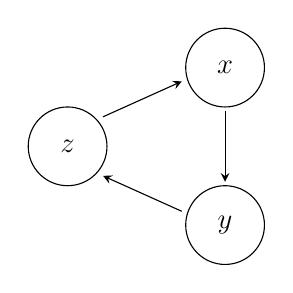
\begin{tikzpicture}[scale=0.5, transform shape]
        % before suppression of alternative
        \draw (5,-2) circle (1) ;
        \draw (5,-2) node{\huge{$y$}};
        \draw (5,2) circle (1) ;
        \draw (5,2) node{\huge{$x$}};
        \draw (1,0) circle (1) ;
        \draw (1,0) node{\huge{$z$}};
        \draw [>=stealth,->] (1.90,0.75) -- (3.90,1.65);
        \draw [>=stealth,->] (3.90,-1.65)-- (1.90,-0.75) ;
        \draw [>=stealth,->] (5,0.9)    -- (5,-0.9) ;
        %\draw [>=stealth,->] (1,2.25) -- (3,3.75);
        % after deletion of a2
        \end{tikzpicture}
   \end{center}
\end{minipage}%
\caption{Example of non transitive preferences matrix and its graphical representation} \label{fig:untransitive_matrix}
\label{fig:untransitive_pref_example}
\end{figure}

In this illustration we can see that alternative $x$ is pairwise preferred over $y$, which is preferred over $z$, which is itself preferred over $x$.
One can easily figure out why it will not been possible to build a complete ranking which is not susceptible to rank reversals. 
Suppose the method, for instance, makes the following ranking:
\begin{equation}
  x \succ y \succ z
  \label{eq:ranking_3alt}
\end{equation}
If alternative $y$ is removed, then the method will logically change the ranking to:
\begin{equation}
  z \succ x 
\end{equation}
and a rank reversal will have happened.\\

The possibility of rank reversals to occur with a method can be problematic. 
Suppose for example that the three alternatives $x$, $y$ and $z$ were three countries which are the final candidates for the hosting of the $2024$ edition of the Olympic Games. 
The candidate which may host the competition would be the one ranked first by the considered method (suffering from rank reversals). An initial ranking could be the one indicated in equation \ref{eq:ranking_3alt}. 
Imagine now, that a large-scale doping scandal is discovered in the country $y$, and that $y$ gets eliminated of the competition. A new candidate, $t$ could then be reselected from the already eliminated ones.

The new pairwise preferences could lead to the following matrix:

\begin{figure}[h]
\begin{minipage}{.2\textwidth}
    \begin{equation*}
        \Pi   = \bordermatrix{~ & x    & z    & t   \cr
                            x & 0    & 0    & 1   \cr
                            z & 1    & 0    & 1   \cr
                            t & 0    & 0    & 0   \cr}
    \end{equation*}
\end{minipage}
\begin{minipage}{.2\textwidth}
    \begin{center}
     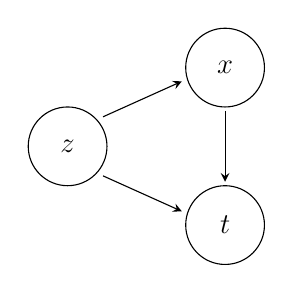
\begin{tikzpicture}[scale=0.5, transform shape]
        % before suppression of alternative
        \draw (5,-2) circle (1) ;
        \draw (5,-2) node{\huge{$t$}};
        \draw (5,2) circle (1) ;
        \draw (5,2) node{\huge{$x$}};
        \draw (1,0) circle (1) ;
        \draw (1,0) node{\huge{$z$}};
        \draw [>=stealth,->] (1.90,0.75) -- (3.90,1.65);
        \draw [>=stealth,->] (1.90,-0.75)-- (3.90,-1.65) ;
        \draw [>=stealth,->] (5,0.9)    -- (5,-0.9) ;
        %\draw [>=stealth,->] (1,2.25) -- (3,3.75);
        % after deletion of a2
        \end{tikzpicture}
   \end{center}
\end{minipage}%
\caption{Example of rank reversal between $x$ and $z$}
\label{fig:transitive_pref_example}
\end{figure}

The ranking method would probably now produce the following ranking:
\begin{equation}
  z \succ x \succ t
  \label{eq:ranking_3alt_t}
\end{equation}

We can conclude from this example that a rank reversal between alternatives $x$ and $z$ occurred due to the removal of alternative $y$. This has some significant consequences since the country $x$ will not be selected as hosting country for the Olympic Games. It is not easy to find reasons why such rank reversals could occur (why should alternative $y$ influence the relative ordering between $x$ and $z$). Such situations are undesirable for most of the decision makers. They will therefore try to avoid multi-criteria methods where rank reversals occur.

For these reasons, two variations of the \textsc{promethee ii} methods have been proposed which were aimed at reducing, or suppressing these rank reversals. The main results of the investigation of these two methods is summarised here under.

\section{\textsc{robust promethee}}


The \textsc{robust promethee} method has originally been proposed by De Smet in \cite{RobPII}. 

It is based on the repetition, $R$ times, of \textsc{promethee ii} on samplings of size $m$. All the repetitions are used to build a probability matrix $P$ which elements $p_{ij}$ represent the probability that an alternative $a_i$ would be ranked before $a_j$ in one random subset. This probability matrix is then used to build a complete ranking. \textsc{robust promethee} is therefore also a ranking method based on pairwise comparisons, but it is hoped that the matrix $P$ will be more transitive than $\Pi$ and that there will therefore be less rank reversals.

Some empirical tests have been performed to verify this assertion on random samples of alternatives taken from the \textsc{epi}\cite{EPI}, \textsc{hdi}\cite{HDI} and \textsc{shanghai}\cite{SHA} data sets.
The results of these tests show that \textsc{robust promethee} indeed seems to reduce the quantity of rank reversals, but only when used with appropriate values of $m$. Furthermore, these appropriate values of $m$ depend on the set of alternatives on which the method is applied and can vary from $30$ to $80 \%$ quantity of alternatives of the problem. This could be a serious obstacle in the practical usage of this method.

\section{\textsc{referenced promethee}}

\textsc{referenced promethee} is the second variation of \textsc{promethee ii} which has been analysed.
It has initially been proposed by Doan and De Smet in \cite{RefPII}.

This method is not a ranking method based on pairwise comparisons, but compares each alternative of the problem to a predefined set of reference profiles.
This method therefore does not suffer from rank reversals: the alternatives are ranked according to a score computed with fixed reference profiles, each alternative's score is therefore independent of any other alternative.

Unfortunately, this method comes with the additional cost of having to find a set of reference profiles. 
It has been seen in the master thesis, that the rankings produced with \textsc{referenced promethee} were strongly dependent on these sets of profiles. Furthermore, it has been seen that it is generally possible to produce rankings similar to the one produced by \textsc{promethee ii} using only few reference profiles (the rankings produced by \textsc{promethee ii} can be considered as satisfactory).

Two techniques aimed at finding sets of reference profiles were studied in the master thesis, but none of them is providings sets of reference producing ``\textsc{promethee ii}-similar'' rankings for all decision problems.


% An example of a floating figure using the graphicx package.
% Note that \label must occur AFTER (or within) \caption.
% For figures, \caption should occur after the \includegraphics.
% Note that IEEEtran v1.7 and later has special internal code that
% is designed to preserve the operation of \label within \caption
% even when the captionsoff option is in effect. However, because
% of issues like this, it may be the safest practice to put all your
% \label just after \caption rather than within \caption{}.
%
% Reminder: the "draftcls" or "draftclsnofoot", not "draft", class
% option should be used if it is desired that the figures are to be
% displayed while in draft mode.
%
%\begin{figure}[!t]
%\centering
%\includegraphics[width=2.5in]{myfigure}
% where an .eps filename suffix will be assumed under latex, 
% and a .pdf suffix will be assumed for pdflatex; or what has been declared
% via \DeclareGraphicsExtensions.
%\caption{Simulation results for the network.}
%\label{fig_sim}
%\end{figure}

% Note that the IEEE typically puts floats only at the top, even when this
% results in a large percentage of a column being occupied by floats.


% An example of a double column floating figure using two subfigures.
% (The subfig.sty package must be loaded for this to work.)
% The subfigure \label commands are set within each subfloat command,
% and the \label for the overall figure must come after \caption.
% \hfil is used as a separator to get equal spacing.
% Watch out that the combined width of all the subfigures on a 
% line do not exceed the text width or a line break will occur.
%
%\begin{figure*}[!t]
%\centering
%\subfloat[Case I]{\includegraphics[width=2.5in]{box}%
%\label{fig_first_case}}
%\hfil
%\subfloat[Case II]{\includegraphics[width=2.5in]{box}%
%\label{fig_second_case}}
%\caption{Simulation results for the network.}
%\label{fig_sim}
%\end{figure*}
%
% Note that often IEEE papers with subfigures do not employ subfigure
% captions (using the optional argument to \subfloat[]), but instead will
% reference/describe all of them (a), (b), etc., within the main caption.
% Be aware that for subfig.sty to generate the (a), (b), etc., subfigure
% labels, the optional argument to \subfloat must be present. If a
% subcaption is not desired, just leave its contents blank,
% e.g., \subfloat[].


% An example of a floating table. Note that, for IEEE style tables, the
% \caption command should come BEFORE the table and, given that table
% captions serve much like titles, are usually capitalized except for words
% such as a, an, and, as, at, but, by, for, in, nor, of, on, or, the, to
% and up, which are usually not capitalized unless they are the first or
% last word of the caption. Table text will default to \footnotesize as
% the IEEE normally uses this smaller font for tables.
% The \label must come after \caption as always.
%
%\begin{table}[!t]
%% increase table row spacing, adjust to taste
%\renewcommand{\arraystretch}{1.3}
% if using array.sty, it might be a good idea to tweak the value of
% \extrarowheight as needed to properly center the text within the cells
%\caption{An Example of a Table}
%\label{table_example}
%\centering
%% Some packages, such as MDW tools, offer better commands for making tables
%% than the plain LaTeX2e tabular which is used here.
%\begin{tabular}{|c||c|}
%\hline
%One & Two\\
%\hline
%Three & Four\\
%\hline
%\end{tabular}
%\end{table}


% Note that the IEEE does not put floats in the very first column
% - or typically anywhere on the first page for that matter. Also,
% in-text middle ("here") positioning is typically not used, but it
% is allowed and encouraged for Computer Society conferences (but
% not Computer Society journals). Most IEEE journals/conferences use
% top floats exclusively. 
% Note that, LaTeX2e, unlike IEEE journals/conferences, places
% footnotes above bottom floats. This can be corrected via the
% \fnbelowfloat command of the stfloats package.




\section{Conclusion}
The problem of the rank reversal phenomenon is a complex problem and the issue of it's legitimacy is still addressed by numerous authors \cite{Brans2016}. 
Nevertheless, two variations of \textsc{promethee ii} aimed at avoiding rank reversal were analysed in the master thesis. Both of them succeed in reducing the rank reversal occurrences. There are also serious obstacles for the practical utilisation of  both these methods which consist in the selection of appropriate values for their respective parameters (the size of the samplings and the sets of reference profiles).

\bibliographystyle{plain}
\bibliography{bibli}
\end{document}

